\chapter{Gnutella vs TorTella}
Gnutella è un protocollo per la ricerca distribuita. Sebbene tale protocollo  supporti un paradigma di ricerca tradizionale del tipo client / server centralizzato, ciò che lo differenzia da altri protocolli è la sua architettura decentralizzata. In questo modello ogni client è un server e viceversa, proprio per questo ogni entità è chiamata servent. Questi forniscono un’interfaccia lato client tramite la quale gli utenti possono inoltrare query e vedere i risultati della ricerca e allo stesso tempo accettano anche query da altri serventi. Una rete di serventi che implementa il protocollo Gnutella è altamente tollerante ai guasti grazie alla sua natura distribuita, poiché se un sottoinsieme di serventi dovesse subire un guasto, le operazioni della rete non verrebbero comunque interrotte.
\section{Protocollo Gnutella}
Il protocollo Gnutella\footnote{Protocollo versione 0.4} definisce il modo in cui i serventi comunicano attraverso la rete. Esso consiste in un insieme di descrittori utilizzati per la comunicazione dei dati attraverso i serventi ed un insieme di regole che governano lo scambio di questi descrittori, che sono:
\begin{description}
\item[Ping] è utilizzato per la scoperta di host nella rete. Un peer ricevente un Ping risponderà con uno o più descrittori di tipo Pong.
\item[Pong] è la risposta ad un descrittore di tipo Ping. Include l’indirizzo di un servente Gnutella connesso e le informazioni riguardanti la quantità dei dati che esso rende disponibile nella rete.
\item[Query] è il meccanismo primario per la ricerca su reti distribuite. Un peer ricevente un descrittore di tipo Query risponderà con un QueryHit se la ricerca sul data set locale fornirà dei risultati.
\item[QueyHit] è la risposta ad un descrittore di tipo Query. Il descrittore fornisce al destinatario abbastanza informazioni per acquisire i dati che soddisfano la Query corrispondente.
\item[Push] un meccanismo che consente ad un servent sotto firewall di contribuire coi suoi dati.
\end{description}
 \begin{figure}
 \centering
 \subfigure[Ping-Pong routing]
   {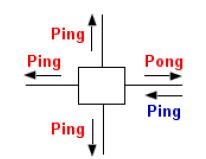
\includegraphics[scale=0.7]{etc/pingpong.jpg}
	\label{pingpong}}
 \hspace{5mm}
 \subfigure[Query-QueryHit routing]
   {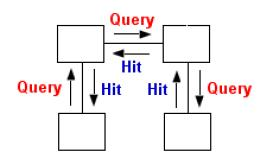
\includegraphics[scale=0.7]{etc/queryqueryhit.jpg}
	\label{queryqueryhit}}
 \end{figure}
I messaggi di Pong e di QueryHit vengono inviati tramite backward routing, ovvero i descrittori seguono lo stesso percorso dei rispettivi descrittori ping/query a ritroso. Il backward routing viene individuato tramite gli identificatori univoci dei messaggi, questo implica che se un servente dovesse ricevere un descrittore di tipo pong/queryhit con id pari a N e questi non abbia ricevuto precedentemente un descrittore di tipo ping/query con id pari a N il pacchetto verrebbe scartato.
\section{Protocollo TorTella}
Il protocollo TorTella nasce prendendo spunto da Gnutella, a cui sono state apportate delle modifiche per renderlo in linea alle necessità dell’applicativo sviluppato. L’architettura adottata da TorTella è stata inizialmente di tipo decentralizzata ibrida, ma vista la presenza di un point of failure a causa della presenza di un server centrale dedicato alle registrazioni, si è deciso di migrare verso un’architettura di tipo completamente decentralizzata. 
Di seguito si riportano alcune caratteristiche del protocollo TorTella, le analogie e le differenze con Gnutella:
\subsection{Descrittori TorTella}
Il protocollo realizzato eredita da Gnutella alcuni descrittori e ne definisce di nuovi per far fronte alle esigenze dell’applicazione:
\begin{description}
\item[Ping] a differenza del descrittore originario non viene inviato in flooding, ma indirizzato verso un unico peer. Viene utilizzato per stabilire nuove connessioni, per notificare i cambiamenti di stato dell'utente e per gestire il meccanismo di failure detection. Composto da due campi, il primo rappresentante il numero di porta e il secondo rappresentante lo status dell’utente. Un pacchetto con un descrittore di tipo Ping conterrà nel campo dati il nickname del peer che lo invia.
\begin{figure}[H]
\begin{center}

\includegraphics[scale=0.7]{etc/ping.jpg}
\caption{Descrittore Ping}
\label{ping}
\end{center}
\end{figure}
\item[Join] viene inviato in flooding per accedere ad una chat creata precedentemente da un generico utente. Contiene dati riguardanti l'utente che ha generato inizialmente il pacchetto, in modo da consentire a tutti i peer riceventi di conoscere tale servente. Contiene il campo status e l’id della chat a cui si vuole connettere, id dell'utente che vuole connettersi, porta e ip del peer mittente, ttl e hops. Il campo dati contiene il nickname.
\begin{figure}[H]
\begin{center}
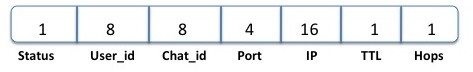
\includegraphics[scale=0.7]{etc/join.jpg}
\caption{Descrittore Join}
\label{join}
\end{center}
\end{figure}
\item[Leave] viene inviato in flooding per notificare l'abbandono di una chat. Contiene l’id della chat room, l'id dell'utente mittente, ttl e hops.
\begin{figure}[H]
\begin{center}
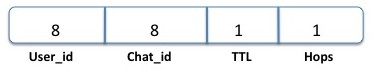
\includegraphics[scale=0.7]{etc/leave.jpg}
\caption{Descrittore Leave}
\label{leave}
\end{center}
\end{figure}
\item[Message] utiizzato per identificare i pacchetti di tipo messaggio. Contiene l’id della chat a cui recapitare il messaggio. Nel campo dati c'è il testo del messaggio.
\begin{figure}[H]
\begin{center}

\includegraphics[scale=0.7]{etc/message.jpg}
\caption{Descrittore Message}
\label{message}
\end{center}
\end{figure}
\item[Search] simile al descrittore Query di Gnutella. Contiene i campi TTL e hops. Nel campo dati è contenuta la stringa di ricerca.
\item[Searchhits] simile al descrittore QueryHit di Gnutella; contiene inoltre, la lista degli utenti partecipanti alle chat rispondenti alla richiesta. Contiene il numero di chat trovate sulla base della query inserita. Il campo dati contiene i risultati della ricerca.
\begin{figure}[H]
\begin{center}

\includegraphics[scale=0.7]{etc/search.jpg}
\caption{Descrittore Search}
\label{search}
\end{center}
\end{figure}
\begin{figure}[H]
\begin{center}

\includegraphics[scale=0.7]{etc/searchhits.jpg}
\caption{Descrittore SearchHits}
\label{searchhits}
\end{center}
\end{figure}
\item[List] serve per richiedere la lista degli utenti connessi ad una specifica chat (non più utilizzato perchè gestito dalla Search). Composto dall’id della chat, ttl e hops.
\item[ListHits] serve per ritornare la lista degli utenti connessi ad una specifica chat (non più utilizzato perchè gestito dalla SearchHits). Composo da il numero di utenti, l'id della chat, ttl e hops. Nel campo dati c'è l'elenco degli utenti della chat.
\begin{figure}[H]
\begin{center}
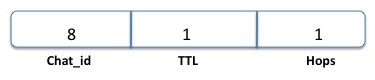
\includegraphics[scale=0.7]{etc/list.jpg}
\caption{Descrittore List}
\label{list}
\end{center}
\end{figure}
\begin{figure}[H]
\begin{center}
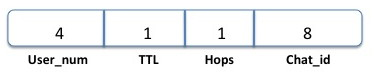
\includegraphics[scale=0.7]{etc/listhits.jpg}
\caption{Descrittore ListHits}
\label{list}
\end{center}
\end{figure}
\item[Bye] serve per sconnettersi da uno specifico peer.
\end{description}

\subsection{Pacchetto TorTella}
Il pachetto TorTella è incluso nel campo dati HTTP ed è composto da 3 campi: un header di 40 byte, un campo descriptor e un campo relativo ai dati di dimensione variabile.
\begin{figure}[H]
\begin{center}

\includegraphics[scale=0.38]{etc/tortellapacket.jpg}
\caption{Pacchetto TorTella}
\label{tortellapacket}
\end{center}
\end{figure}
Si presentano di seguito l’header utilizzato per la realizzazione del protocollo utilizzato e quello Gnutella:
\begin{figure}[H]
\begin{center}
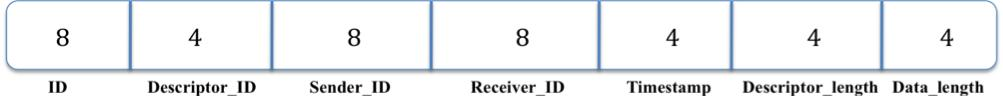
\includegraphics[scale=0.38]{etc/tortellaheader.jpg}
\caption{Header TorTella}
\label{tortellaheader}
\end{center}
\end{figure}
\begin{description}
\item[ID] un unsigned long long (8 byte) che identifica il pacchetto in modo univoco;
\item[Descriptor\_ID] un unsigned int (4 byte) che specifica il descrittore di pacchetto trasportato;
\begin{itemize}
	\item 0x01: Ping
	\item 0x03 = List
	\item 0x04 = ListHits
	\item 0x05 = Join
	\item 0x06 = Leave
	\item 0x07 = Message
	\item 0x09 = Search
	\item 0x10 = SearchHits
	\item 0x11 = Bye
	\item 0x12 = Close (utilizzato localmente)
\end{itemize}
\item[Sender\_ID] un unsigned long long (8 byte) che identifica in modo univoco il mittente del pacchetto;
\item[Receiver\_ID] un unsigned long long (8 byte) che identifica in modo univoco il destinatario del pacchetto;
\item[Timestamp] un time\_t (4 byte) che indica l’ora in cui il pacchetto è stato inviato;
\item[Descriptor\_length] un unsigned int (4 byte) che indica la lunghezza del descrittore che segue l’header;
\item[Data\_length] un unsigned int (4 byte) che indica la lunghezza del campo dati presente all’interno del pacchetto.
\end{description}
\begin{figure}[H]
\begin{center}
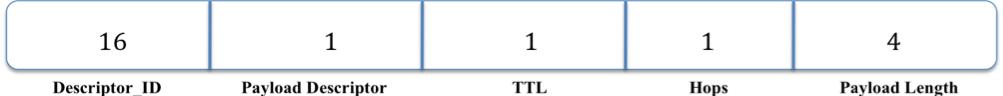
\includegraphics[scale=0.38]{etc/gnutellaheader.jpg}
\caption{Header Gnutella}
\label{gnutellaheader}
\end{center}
\end{figure}
\begin{description}
\item[Descriptor\_ID] una stringa di 16 byte che identifica univocamente il descrittore sulla rete;
\item[Payload Descriptor]
\begin{itemize}
	\item 0x00 = Ping
	\item 0x01 = Pong
	\item 0x40 = Push
	\item 0x80 = Query
	\item 0x81 = QueryHits	
\end{itemize}
\item[TTL] Time to live. Il numero di volte che il descrittore sarà inoltrato dai serventi Gnutella prima che esso sia rimosso dalla rete. Ogni servente decrementerà il TTL prima di inoltrarlo ad un altro servente. Quando il TTL è pari a zero, il descrittore non verrà più inoltrato;
\item[Hops] Il numero di volte che il descrittore è stato inoltrato. Il TTL e il campo Hops devono soddisfare la seguente condizione: 
\begin{center}
\texttt{TTL(0) = TTL(i)  + Hops(i)}
\end{center}
\item[Payload Length] La lunghezza del descrittore successivo a quest’header. Il prossimo descriptor header si trova esattamente Payload Length bytes dalla fine di questo header.
\end{description}
Come si può notare, l’header TorTella non presenta i campi TTL e Hops poiché questi servono solo ed esclusivamente nel caso di invio di pacchetti di flooding, quindi si è pensato di collocare questi due campi all’interno del campo descriptor; inoltre vengono aggiunti i campi sender\_id e receiver\_id per gestire al meglio l’invio e la ricezione dei pacchetti. Il campo descrittore presenta una lunghezza variabile a seconda del descriptor\_id presente nell’header.